\section{Speeding Up the Naive Algorithm}

The naive exact matching algorithm is stupid. It always shifts $P$ by only one even if it knows for sure that the next shift will not yield a match. This gives us some ideas on how to improve the algorithm. If we can shift $P$ by more than one character, but never shift so far as to miss the next occurrence of $P$ in $T$, we can improve the runtime of the naive algorithm.

Doing this, however, requires us to have some prior knowledge of the pattern $P$ or the text $T$.

\section{Foundamental Preprocessing}

A fundemental preprocessing is a generalized way to process the pattern $P$ to gain knowledge of the pattern, independent of any particular algorithm.

\begin{definition}
    Given a string $S$ and a position $i>1$, let $Z_i(S)$ be the length of the longest substring of $S$ that starts at $i$ and matches a prefix of $S$.

    In other words, $Z_i(S)$ is the length of the longest prefix of $S[i\ldots |S|]$ that matches a prefix of $S$.
\end{definition}

\begin{definition}[Z-box] \index{Z-box}
    For any position $i > 1$ where $Z_i$ is greater than 0, the \textbf{Z-box} at $i$ is the interval starting at $i$ and ending at $i+Z_i-1$.
\end{definition}

\begin{marginfigure}
    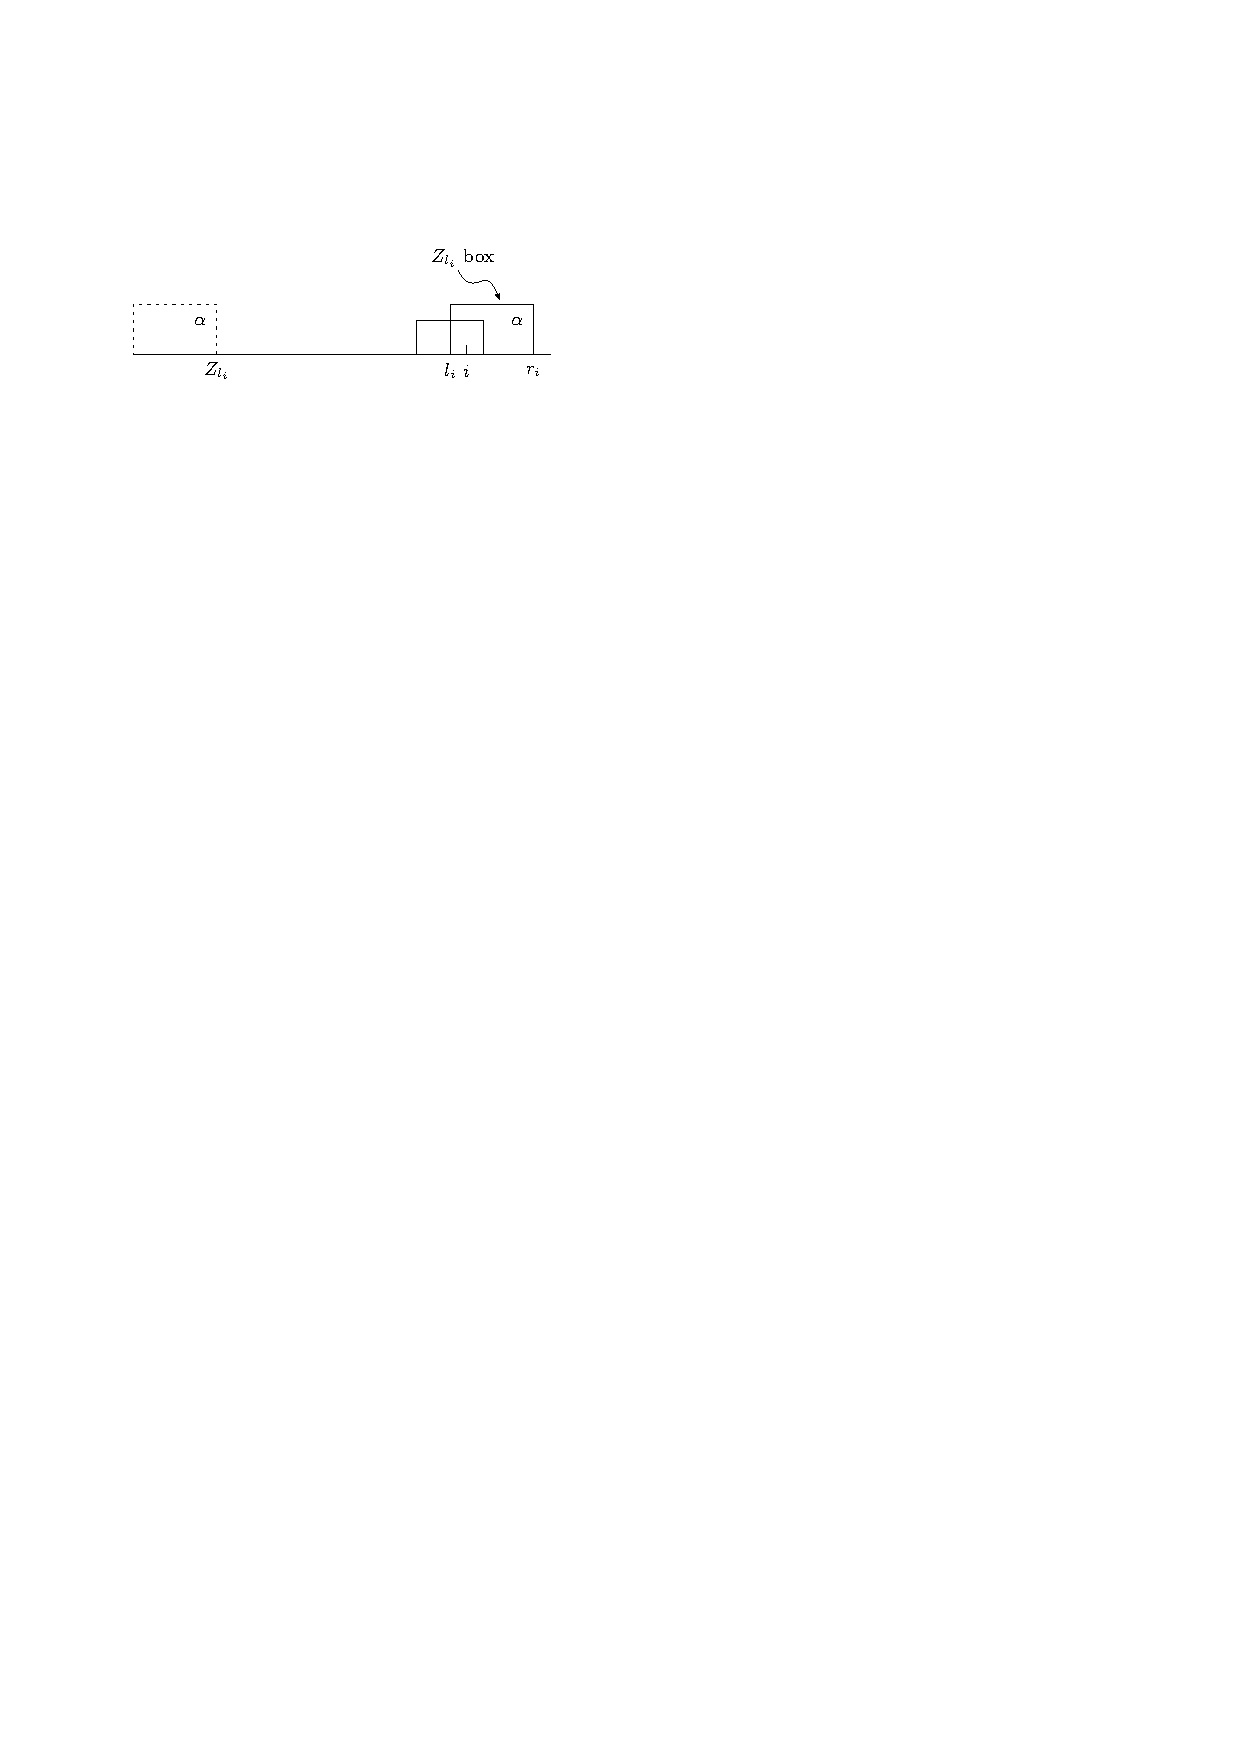
\includegraphics[width=\linewidth]{z/z-box.pdf}
    \caption{Relations between $i$, $l_i$, $r_i$ and the Z-box at $l_i$.}
    \label{fig:z-box}
\end{marginfigure}

\begin{definition}
    For every $i > 1$, $r_i$ is the right endpoint of the Z-box that begins at or befor position $i$ (i.e. the closest Z-box to the left). More formally, $r_i$ is the largest value of $j + Z_j - 1$ over all $1 < j \leq i$ such that $Z_j > 0$.
\end{definition}

\begin{codebox}
    \Procname{$\proc{Compute-Z}(S)$}
    \li $n = |S|$
    \li $Z = \text{empty array of length $n$}$ 
\end{codebox}